\chapter{Efficient Conflict Detection of Change-based Models}
\label{ch:conflict_detection}
  
Comparison -- difference identification and conflict detection -- of large models can be time-consuming since every element has to be visited, matched, and compared with its respective element in other models. This can result in bottlenecks in collaborative modelling environments, where identifying differences between two versions of a model is desirable. Reducing the comparison process to only the elements that have been modified since a previous known state (e.g. previous version) could significantly reduce the time required for large model comparison. This paper presents how change-based persistence can be used to localise the comparison of models so that only elements affected by recent changes are compared and to substantially reduce comparison and differencing time (up to 90\% in some experiments) compared to state-based model comparison. 

\section{Another Running Example}
\label{sec:another_running_example}
In this section, we introduce another running example to explain how to detect conflicts using the element tree. We use this example to construct a new element tree and to explain how conflict detection is performed in EMF Compare, EMF Store, and our change-based conflict detection. Let's say that there is a project to develop a Role Playing Game (RPG). Jane, as the technical leader, set up the initial model. The records of events during setting up the initial is recorded in the CBP in List. \ref{fig:class_diagram_origin}. From the List., we know that she created a class \textsf{Character} that contains an operation \textsf{attack} with three parameters: \textsf{gem}, \textsf{target}, and \textsf{weapon} (lines 1-14). She also created four other classes; \textsf{Troll} (lines 15-16), \textsf{Giant} (lines 17-21), \textsf{Knight} (lines 22-26), and \textsf{Mage} (lines 27-28). She then pushed her work to a change-based version control system. If her work is visualised in state-based format, the model looks like in Fig. \ref{fig:class_diagram_origin}.

\vspace{-15pt}
\begin{lstlisting}[firstnumber=1,style=eol,caption={The recorded events to produce the original model in Fig. \ref{fig:class_diagram_origin} (original version).},label=lst:cbp_origin]
create character type Class
set character.name to "Character" 
create attack type Operation
set attack.name to "attack" 
add attack to character.operations at 0
create gem type Parameter
set gem.name to "gem" 
add gem to attack.parameters at 0
create target type Parameter
set target.name to "target" 
add target to attack.parameters at 1
create weapon type Parameter
set weapon.name to "weapon" 
add weapon to attack.parameters at 2
create troll type Class
set troll.name to "Troll" 
create giant type class
set giant.name to "Giant"
create cast type Operation
set cast.name to "smash"
add cast to giant.operations at 0
create knight type Class
set knight.name to "Knight"
create smash type Operation
set smash.name to "smash"
add smash to knight.operations at 0
create mage type Class
set mage.name to "Mage" 
\end{lstlisting}

She then assigned this work to Bob and Alice. Both of them checked out this project to their own machine. Alice then started to continue the model. She then moved parameter \textsf{target} to the first place in operation \textsf{attack}'s parameters, because she thought it was more intuitive for programmers to think about the \textsf{target} first than the rest parameters (List. \ref{lst:cbp_right}, line 29). She also moved operations \textsf{smash} from class \textsf{Knight} to class \textsf{Giant} and \textsf{cast} from class \textsf{Giant} to class \textsf{Mage} as thy are more reasonable to belong to their new classes (lines 30-33). Alice also created a generalisation relationship with id \textsf{rightGen} from class \textsf{Troll} to class \textsf{Character} (34-36). Bob also did the same thing except that his generalisation came with id \textsf{leftGen} (List. \ref{lst:cbp_left}, line 29-31). 

Later on, Jane then informed them that she wanted all good characters should be derived from a general, hero-like class, and the enemy should be the Orcs not Trolls. She also instructed that Bob should focus on developing class \textsf{Knight} and Alice on class \textsf{Mage}. In consequence, Alice then changed the name of class \textsf{Character} from ``Character'' to ``Hero'' (the id of class \textsf{Hero} is still \textsf{character}) (line 37). Again, Bob did the same thing. He also changed the name of class \textsf{Character} from ``Character'' to ``Hero'' (line 32). Instead of creating a new generalisation relationship, both of them preferred to move the generalisation relationships that they had created to their assigned classes. Alice moved generalisation \textsf{rightGen} from class \textsf{Troll} to class \textsf{Mage} (lines 38-39), and Bob move generalisation \textsf{leftGen} from class \textsf{Troll} to class \textsf{Knight} (lines 33-34). Bob also moved parameter \textsf{target} in operation \textsf{attack} to the last index as he thought setting target as the last parameter was intuitive (line 35), and deleted the class {Giant}, and unfortunately, he deleted class \text{Giant} accidentally (lines 36-40). The class diagrams of Bob and Alice's models are visualised in Figures \ref{fig:class_diagram_left} and \ref{fig:class_diagram_right} respectively. Lastly, Alice changed the \textsf{name} of class \textsf{Troll} to ``Orc'' (line 40) while Bob changed it to ``Ogre'' (line 41).  

\vspace{-15pt}
\begin{lstlisting}[firstnumber=29,style=eol,caption={The appended events made by Alice to produce the right model in Fig. \ref{fig:class_diagram_right} (right version).},label=lst:cbp_right]
move target in attack.parameters from 1 to 0
remove smash from knight.operations at 0 composite l1
add smash to giant.operations at 0 composite l1
remove cast from giant.operations at 1 composite l2
add cast to mage.operations at 0 composite l2
create rightGen type Generalization
set rightGen.general to character
set troll.generalization to rightGen
set character.name from "Character" to "Hero"
remove rightGen from troll.generalization composite l3
set mage.generalization to rightGen composite l3
set troll.name from "Troll" to "Orc"
\end{lstlisting}

\vspace{-15pt}
\begin{lstlisting}[firstnumber=29,style=eol,caption={The appended events made by Bob to produce the left model in Fig. \ref{fig:class_diagram_left} (left version).},label=lst:cbp_left]
create leftGen type Generalization
set leftGen.general to character
set troll.generalization to leftGen
set character.name from "Character" to "Hero"
remove leftGen from troll.generalization composite r1
set knight.generalization to leftGen composite r1
move target in attack.parameters from 1 to 2
unset cast.name from "cast" to null composite r2
remove cast from giant.operations at 0 composite r2
delete cast composite r2
unset giant.name from "Giant" to null composite r2
delete giant comp r2
set troll.name from "Troll" to "Ogre"
\end{lstlisting}

In Listings \ref{lst:cbp_right} and \ref{lst:cbp_left}, we also introduce composite events -- lines with keyword \textsf{composite} -- that represent composite operations. 
Composite operations are operations that should be treated as one composition -- identified with the same composite id. 
For example, moving an element from a container to another container is composite event since it consists of two operations: 
removing/unsetting the element from its source container and adding/setting it to its target container (lines 36-37 Listing \ref{lst:cbp_right}). 
Using the information contained in CBPs in Listings in CBPs in Listings \ref{lst:cbp_right} and \ref{lst:cbp_left}, 
we can construct an element tree as depicted in Fig. \ref{fig:element_tree_game} using the element tree construction method presented in Section \ref{sec:tree_construction}. 

\begin{figure*}
    \centering
    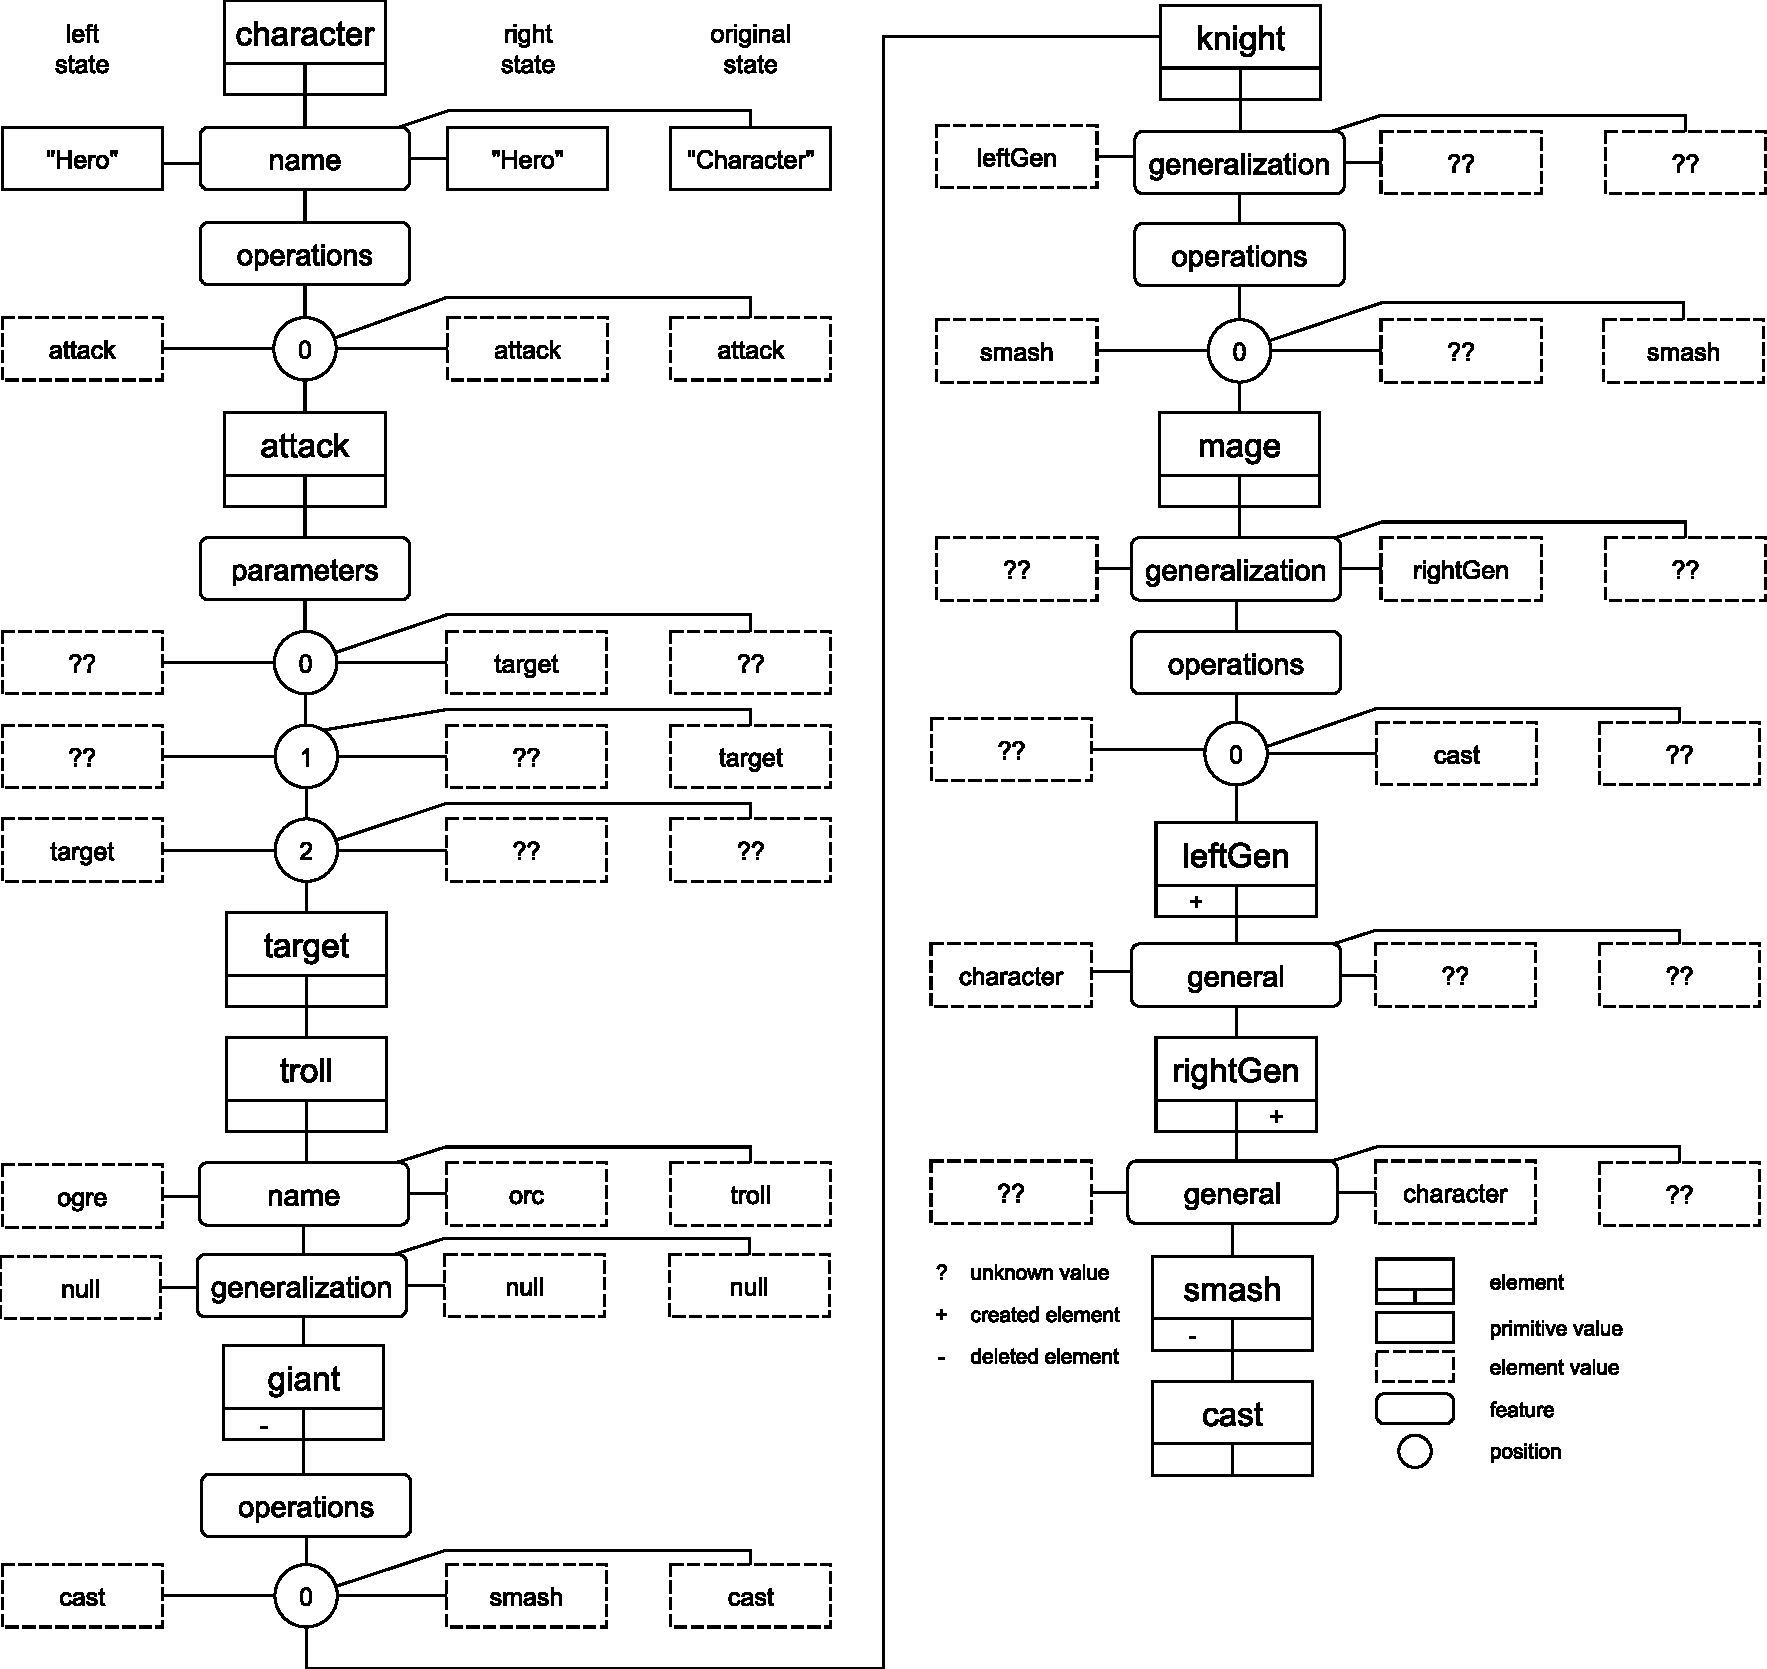
\includegraphics[width=\linewidth]{element_tree_game}
    \caption{An element tree constructed using information contained in CBPs in Listings \ref{lst:cbp_right} and \ref{lst:cbp_left}.}
    \label{fig:element_tree_game}
\end{figure*} 

During the the construction of the element tree, these events in Listings \ref{lst:cbp_right} and \ref{lst:cbp_left} are registered to the affected elements, features, and values. 
This registration forms one-to-many relationships between keys and the events. 
The keys are \textsf{element} for elements, \textsf{element-feature} for single-valued features, and \textsf{element-feature-value} for multivalued-features.
With this mapping, we can trace all events that affects certain elements, features, and values. 
The mapping of the events in Listings \ref{lst:cbp_right} and \ref{lst:cbp_left} is in Table \ref{tab:keyeventsmap}.

\begin{table}[]
    \centering
    \caption{The mapping of elements, features, and values in Fig. \ref{fig:element_tree_game} to the events that affects them.}
    \label{tab:keyeventsmap}
    \begin{scriptsize}
        \begin{tabular}{|m{0.38\linewidth}|m{0.23\linewidth}|m{0.23\linewidth}|}
            \hline
            \textbf{Key} & \textbf{Left Events} & \textbf{Right Events} \\ \hline
            character                          & ol30, ol32                                & or35, or37                                 \\ \hline
            character.name                     & ol32                                      & or37                                       \\ \hline
            attack                             & ol35                                      & or29                                       \\ \hline
            attack.parameters.target           & ol35                                      & or29                                       \\ \hline
            target                             & ol35                                      & or29                                       \\ \hline
            troll                              & ol31, ol33                                & or36, or38                                 \\ \hline
            troll.name                         & ol41                                      & or40                                       \\ \hline
            troll.generalization               & ol31, ol33                                & or36, or38                                 \\ \hline
            giant                              & ol37, ol38, ol39, ol40                    & or31, or32                                 \\ \hline
            giant.name                         & ol38                                      &                                            \\ \hline
            giant.operations.cast              & ol37                                      & or32                                       \\ \hline
            giant.operations.smash             &                                           & or31                                       \\ \hline
            knight                             & ol34                                      & or30                                       \\ \hline
            knight.generalization              & ol34                                      &                                            \\ \hline
            knight.operations.smash            &                                           & or30                                       \\ \hline
            mage                               &                                           & or33, or39                                 \\ \hline
            mage.generalization                &                                           & or39                                       \\ \hline
            mage.operations.cast               &                                           & or33                                       \\ \hline
            leftGen                            & ol29, ol30, ol31, ol33, ol34              &                                            \\ \hline
            leftGen.general                    & ol30                                      &                                            \\ \hline
            rightGen                           &                                           & or34, or35, or36, or38, or39               \\ \hline
            rightGen.general                   &                                           & or35                                       \\ \hline
            smash                              &                                           & or30, or31                                 \\ \hline
            cast                               & ol36, ol37, ol38                          & or32, or33                                 \\ \hline
            cast.name                          & ol36                                      &                                            \\ \hline
        \end{tabular}
        o: operation; l: left side; r: right side; n: line number in the listing
    \end{scriptsize}
\end{table}

\section{Conflict Detection}
\label{sec:conflict_detection}
In state-based model comparison, a conflict detection usually requires two different versions of a model and one shared ancestor -- the original version. In change-based model comparison, the original version is not required since it is implicitly contained in the other two versions' change-based persistence. A conflict occurs when an element is identified changed in both versions in reference to its original version. A conflict also occurs when a change from a version is applied first causes another change from the other version cannot be applied due to dependency violation. 

Let's say that we have three versions of a model: $m_{o}$ is the original version, $m_{l}$ is the left version, and $m_{r}$ is the right version, where $m_{o}$, $m_{l}$, $m_{r}$ $\in$ $M$. 
Every model consists of elements. Thus, $E_{O}$, $E_{L}$ , and $E_{R}$ are sets of elements of models $M_{O}$, $M_{L}$, and $E_{R}$ respectively, where $E_{O}=\{e_{o1}, e_{o2}, ..., e_{oa}\}$, $E_{L}=\{e_{l1}, e_{l2}, ..., e_{lb}\}$, and $E_{R}=\{e_{r1}, e_{r2}, ..., e_{rc}\}$. Since we detect conflicts up to the level of values in features, an $e$ can also refer to a feature or feature's value instead of only referring to an element. We also have two sets of operations $O_{L}$ and $O_{R}$ that changes model $m_{m}$ to models $m_{l}$ and $m_{r}$ respectively, where $O_{L}=\{o_{l1}, o_{l2}, ..., o_{ld}\}$ and $O_{R}=\{o_{r1}, o_{r2}, ..., o_{rf}\}$. 

\subsection{State-based Conflict Detection: EMF Compare}
\label{sec:state_based_conflict_detection_emf_compare}
In state-based model comparison, the two sets of operations $O_{L}$ and $O_{R}$ are not readily available. They have to be derived trough model differencing. Both sets can be obtained by differencing $M_{L}$ to $M_{O}$ and $M_{R}$ to $M_{O}$ using an LCS algorithm as explained in Section \ref{sec:model_differencing}. These two differencing processes produce two sets of differences, $D_{OL}$ and $D_{OR}$, where $D_{OL}$ = $\{d_{ol1}$, $d_{ol2}$, ..., $d_{olg}\}$, $D_{OR}$ = $\{d_{or1}$, $d_{or2}$, ..., $d_{orh}\}$, and each difference $d$ is expressed as in (\ref{eq:diff_definition}). These differences can be treated as operations since if we apply these differences as operations to a target model, they transform it to become equivalent to a reference model. For example, applying a set of differences $D_{OL}$ to a model $M_{O}$ will transform it to model $M_{L}$. Therefore, we can say that these differences are equivalent to operations. Thus, we can have two sets of operations, $O_{L}$ and $O_{R}$, which $O_{L} \equiv D_{OL}$ and $O_{R} \equiv D_{OR}$. These operations can then be used to detect conflicts using (\ref{eq:conflict_1.8}), (\ref{eq:conflict_1.9}), and (\ref{eq:conflict_1.10}).  

If we use EMF Compare to derive $O_{L}$ from Bob's and Jane's versions in Fig. \ref{fig:class_diagram_rpg} and present it in the format of change events, we obtain the following list. 
\begin{lstlisting}[firstnumber=1,style=eol,caption={The derived change events (operations) made by Bob to produce the right model in Fig. \ref{fig:class_diagram_left} (right version).},label=lst:cbp_left_state]
move target in attack.parameters from 1 to 2
set character.name from "Character" to "Hero"
set troll.name from "Troll" to "Ogre"
create leftGen type Generalization
set leftGen.general to character
set knight.generalization to leftGen
delete cast
delete giant
\end{lstlisting}

And following list is the derived change events for $O_{R}$ that are obtained from Bob's and Jane's versions in Fig. \ref{fig:class_diagram_rpg}. 
\begin{lstlisting}[firstnumber=1,style=eol,caption={The derived change events (operations) made by Alice to produce the right model in Fig. \ref{fig:class_diagram_right} (right version).},label=lst:cbp_right_state]
move gem in attack.parameters from 0 to 1
set character.name from "Character" to "Hero"
set troll.name from "Troll" to "Orc"
remove smash from knight.operations at 0
add smash to giant.operations at 0
create rightGen type Generalization
set rightGen.general to character
set mage.generalization to rightGen
remove cast from giant.operations at 1
add cast to mage.operations at 0
\end{lstlisting}

\textbf{Real Conflict}. In EMF Compare, a conflict occurs between two different operations, $o_{l}$ and $o_{r}$, if each is applied to a same element produce two different eventual states, where $!$ is the operator for expressing that two operations are in conflict. This conflict is classified \textsf{REAL} by EMF Compare.
\begin{equation} \label{eq:conflict_1.8}
e_{o} + o_{l} \not\equiv e_{o} + o_{r} \Rightarrow o_{l}\;!\;o_{r}
\end{equation} 
\textbf{Pseudo Conflict}. A conflict is classified as \textsf{PSEUDO} if the eventual states produced are equivalent. 
\begin{equation} \label{eq:conflict_1.9}
e_{o} + o_{l} \equiv e_{o} + o_{r} \Rightarrow o_{l}\;!_{p}\;o_{r}
\end{equation} 
\textbf{Non-applicability}. A conflict also occurs when applying operation $o_{l}$ to element $e_{o}$ makes $o_{r}$ inapplicable to element $e_{o}$. Therefore, operations $o_{l}$ and $o_{r}$ are in conflict. 
%For instance, Alice moved operation \textsf{smash} from class \textsf{Knight} to class \textsf{Giant} but this class was deleted by Bob. Deleting class \textsf{Giant} makes the move inapplicable. This conflict is classified \textsf{REAL} by EMF Compare.
\begin{equation} \label{eq:conflict_1.10}
(e_{o} + o_{r} \not\equiv e_{o}) \wedge (e_{o} + o_{l} + o_{r} \equiv e_{o} + o_{l}) \Rightarrow o_{l}\;!\;o_{r}
\end{equation}

\begin{table*}[]
    \centering
    \caption{Conflicting change events identified using EMF Compare based on the case in Fig. \ref{fig:class_diagram_rpg}.}
    \label{table:conflicts_emfc}
    % Please add the following required packages to your document preamble:
    % \usepackage[table,xcdraw]{xcolor}
    % If you use beamer only pass "xcolor=table" option, i.e. \documentclass[xcolor=table]{beamer}
    \begin{tabular}{|l|l|l|l|}
        \hline
        \multicolumn{1}{|c|}{{\color[HTML]{000000} \textbf{ID}}} & \multicolumn{1}{c|}{{\color[HTML]{000000} \textbf{Left Change Events (Bob)}}} & \multicolumn{1}{c|}{{\color[HTML]{000000} \textbf{Right Change Events (Alice)}}}                                      & \multicolumn{1}{c|}{{\color[HTML]{000000} \textbf{Type}}}           \\ \hline
        EC1                                                      & set character.name from "Character" to "Hero"                                 & set character.name from "Character" to "Hero"                                                                         & \begin{tabular}[c]{@{}l@{}}pseudo\\conflict\end{tabular} \\ \hline
        EC2                                                      & set troll.name from "Troll" to "Ogre"                                         & set troll.name from "Troll" to "Orc"                                                                                  & \begin{tabular}[c]{@{}l@{}}real conflict\end{tabular}        \\ \hline
        EC3                                                      & delete cast                                                                  & \begin{tabular}[c]{@{}l@{}}remove cast from giant.operations at 1\\ add cast to mage.operations at 0\end{tabular}     & \begin{tabular}[c]{@{}l@{}}non-\\ applicability\end{tabular}        \\ \hline
        EC4                                                      & delete giant                                                                   & \begin{tabular}[c]{@{}l@{}}remove smash from knight.operations at 0\\ add smash to giant.operations at 0\end{tabular} & \begin{tabular}[c]{@{}l@{}}non-\\ applicability\end{tabular}        \\ \hline
    \end{tabular}
\end{table*}

Using (\ref{eq:conflict_1.8}), (\ref{eq:conflict_1.9}), and (\ref{eq:conflict_1.10}) and information in Listings \ref{lst:cbp_right_state} and \ref{lst:cbp_left_state}, we can identify four conflicts -- presented in Table \ref{table:conflicts_emfc} along with their conflicting change events. Conflict \textsf{EC1} is a pseudo duality conflict since both modify the same class \textsf{character}'s feature \textsf{name} resulting the same end states, ``Hero'' or ``Hero''. Conflict \textsf{EC2} is a duality conflict. Applying changing \textsf{troll}'s \textsf{name} to ``Ogre'' and \textsf{troll}'s \textsf{name} to ``Orc'' produces two different states -- ``Ogre'' and ``Orc''. Conflicts \textsf{EC3} and \textsf{EC4} are non-applicability conflicts since if we delete operation \textsf{cast} first then it cannot removed from class \textsf{giant}'s operations to be added to \textsf{mage}'s \textsf{operations}, and if we delete class \textsf{giant} first then operation \textsf{smash} cannot be added to that class' operations.

Conflict detection in state-based comparison might not be accurate since the derived differences/operations might not reflect the real historical changes of a model.
For example, EMF Compare does not detect that Alice and Bob modified the same element -- parameter \textsf{target} -- as indicated by line 29 in List. \ref{lst:cbp_right} and line 35 in List. \ref{lst:cbp_left} . Using an LCS algorithm, the derived operations related to the feature \textsf{parameters} of element \textsf{attack}, which if presented as change events, are expressed as [\texttt{\small \textbf{move} target \textbf{in} attack.parameters \textbf{from} 1 \textbf{to} 2}] for Bob's version and [\texttt{\small \textbf{move} gem \textbf{in} attack. parameters \textbf{from} 1 \textbf{to} 2}] for Alice's version. Using (\ref{eq:conflict_1.3}), both operations are not in conflict since both operations modify two different elements, \textsf{target} and \textsf{gem}. The result is different if we employ change-based approach to detect conflicts using the change event records in Listings \ref{lst:cbp_right} and \ref{lst:cbp_left}. We explain this in Section \ref{sec:change_based_conflict_detection_emf_store}.

\subsection{Change-based Conflict Detection: EMF Store}
\label{sec:change_based_conflict_detection_emf_store}

\textbf{Non-commutability}. In EMF Store \cite{koegel2010emfstore} , operations $o_{l}$ and $o_{r}$ are in conflict if applying them in different order to a same element, in this case element $e_{o}$, produces two different eventual states.
\begin{equation} \label{eq:conflict_1.3}
e_{o} + o_{l} + o_{r} \not\equiv e_{o} + o_{l} + o_{r} \Rightarrow o_{l}\;!\;o_{r}
\end{equation} 
%For example, Alice changed the \textsf{name} of class \textsf{Troll} to ``Orc''while Bob renamed it to ``Ogre'' (Figure \ref{fig:class_diagram_rpg}). Applying Alice's change first to Bob's change results in the class' \textsf{name} equals to ``Ogre'', or ``Orc'' if the order is reversed. 
\textbf{Pseudo non-commutability}. However, after examining the implementation \footnote{\url{https://git.eclipse.org/c/emf-store}}, even though the eventual states are equivalent, both operations are still treated  in conflict. 
\begin{equation} \label{eq:conflict_1.5}
e_{o} + o_{l} + o_{r} \equiv e_{o} + o_{l} + o_{r} \Rightarrow o_{l}\;!_{p}\;o_{r}
\end{equation} 
\textbf{Non-applicability}. This non-applicability rule is the same with the non-applicability rule in the state-based conflict detection. We present the rule again here. 
\begin{equation} \label{eq:conflict_1.6}
(e_{o} + o_{r} \not\equiv e_{o}) \wedge (e_{o} + o_{l} + o_{r} \equiv e_{o} + o_{l}) \Rightarrow o_{l}\;!\;o_{r}
\end{equation}
\textbf{Composite}. If operation $o_{l}$ is in conflict with operation $o_{r}$ where $o_{r}$ is a member of composite operation $co_{r}$ then operation $o_{l}$ is also in conflict with each operation $o_{n}$ in composite operation $co_{r}$.
%For example, deleting class \textsf{Giant} (List. \ref{lst:cbp_left} line 40) is not only in conflict with adding operation \textsf{smash} to class \textsf{Giant}'s operations (List. \ref{lst:cbp_right} line 31), but also with the removal of operation \textsf{smash} from class \text{Knight}'s operations (List. \ref{lst:cbp_right} line 31).
\begin{equation} \label{eq:conflict_1.7}
o_{l}\;!\;o_{r} \wedge o_{r} \in co_{r} \Rightarrow o_{l}\;!\; \forall o_{n} | o_{n} \in co_{r}
\end{equation}

\begin{table*}[]
    \centering
    \caption{Conflicting change events identified using EMF Store in Listings \ref{lst:cbp_right} and \ref{lst:cbp_left}.}
    \label{table:conflicts_emfs}
    \begin{tabular}{|l|l|l|l|}
        \hline
        \multicolumn{1}{|c|}{{\color[HTML]{000000} \textbf{ID}}} & \multicolumn{1}{c|}{{\color[HTML]{000000} \textbf{Left Change Events (Bob)}}}                                                                                                                                              & \multicolumn{1}{c|}{{\color[HTML]{000000} \textbf{Right Change Events (Alice)}}}                                                          & \multicolumn{1}{c|}{{\color[HTML]{000000} \textbf{Type}}}                                    \\ \hline
        \multirow{2}{*}{ES1} & set troll.generalization from null to leftGen                                                                                                                                                                              & \begin{tabular}[c]{@{}l@{}}unset troll.generalization from rightGen to null\\set mage.generalization from null to rightGen\end{tabular} & \multirow{2}{*}{\begin{tabular}[c]{@{}l@{}}non-\\ commutability, \\ composite\end{tabular}}                                                                                             \\ \cline{2-3}
        & \begin{tabular}[c]{@{}l@{}}unset troll.generalization from leftGen to null\\ set knight.generalization from null to leftGen\end{tabular}                                                                                   & set troll.generalization from null to rightGen                                                                                             &  \\ \hline
        ES2                                                      & set character.name from "Character" to"Hero"                                                                                                                                                                               & set character.name from "Character" to "Hero"                                                                                             & \begin{tabular}[c]{@{}l@{}}pseudo non-\\ commutability\end{tabular}                          \\ \hline
        ES3                                                      & move target in attack.parameters from 1 to 2                                                                                                                                                                               & move target in attack.parameters from 1 to 0                                                                                              & \begin{tabular}[c]{@{}l@{}}non-\\ applicability\end{tabular}                                 \\ \hline
        \multirow{2}{*}{ES4} & \multirow{2}{*}{\begin{tabular}[c]{@{}l@{}}unset cast.name from "cast" to null\\ remove cast from giant.operations at 0\\ delete cast type Operation\\ unset giant.name from "Giant" to null\\ delete giant\end{tabular}}                                                                                                                                                                                                                            & \begin{tabular}[c]{@{}l@{}}remove cast from giant.operations at 0\\ add cast to mage.operations at 0 \end{tabular}                         
        & \multirow{2}{*}{\begin{tabular}[c]{@{}l@{}}non-\\ applicability,\\ composite\end{tabular}} \\ \cline{3-3}
        &  & \begin{tabular}[c]{@{}l@{}}remove smash from knight.operations at 0\\ add smash to giant.operations at 1\\ \\ \\ \end{tabular}                     &   \\ \hline
        
        ES5                                                      & set troll.name from "Troll" to "Ogre"                                                                                                                                                                                      & set troll.name from "Troll" to "Orc"                                                                                                      & \begin{tabular}[c]{@{}l@{}}non-\\ commutability\end{tabular}                                 \\ \hline
    \end{tabular}
\end{table*}

In change-based conflict detection, all operations applied to a model are already available in change-based persistence, thus the operations do not need to be derived trough a diffing process. The availability of real historical changes can improve the accuracy of change detection since we can identify precisely elements that have been changed. In consequence, the undetected conflict in state-based conflict detection can be detected. For example, in Listing \ref{lst:cbp_right} line 29, parameter \textsf{target} has been moved from index 1 to 0, while in Listing \ref{lst:cbp_left} line 35, it was moved from index 1 to 2. Since both operations modified the same parameter \textsf{target}, using (\ref{eq:conflict_1.3}) we can identify that both operations are in conflict; parameter \textsf{target} are at different indexes if both operations are applied in different order, and \textsf{parameters}, the containing feature of \textsf{target}, is an ordered feature (Table \ref{table:conflicts_emfs} id ES1).  

The drawback of EMF Store is that it only performs comparison between operations to determine conflicts; it does no take into account the end states of models produced by the operations. In consequence, two operations are in conflict just by modifying a same element regardless of the end states that they produce to the element \cite{DBLP:conf/sfm/BroschKLSWW12}; there is no classification of conflicts to \textsf{REAL} or \textsf{PSEUDO} conflicts. For example, two operations represented by the two change events in Listing \ref{lst:cbp_right} at line 37 and Listing \ref{lst:cbp_right} at line 32, that change the same feature \textsf{name} to the same value ``Hero'', are treated in conflict (Table \ref{table:conflicts_emfs} id ES2). 

The inconsideration of eventual states also causes the assignments of generalizations \textsf{leftGen} and \textsf{rightGen} to class \textsf{troll}'s feature \textsf{generalization}, in Listings \ref{lst:cbp_right} at line 38 and \ref{lst:cbp_left} at line 33, to be in conflict with the \textsf{move} operations on the opposite sides (Table \ref{table:conflicts_emfs} id ES1). Setting feature \textsf{troll}'s \textsf{generalization} to element \textsf{leftGen} is in conflict with the \textsf{move} composite operation that moves \textsf{rightGen} from \textsf{troll}'s \textsf{generalization} to \textsf{mage}'s \textsf{generalization}. Using the non-commutability (\ref{eq:conflict_1.3}) and composite (\ref{eq:conflict_1.7}) rules, we can detect that executing these operations in different order causes \textsf{troll}'s \textsf{generalization} has two different eventual values; \textsf{troll}'s \textsf{generalization} is null if the \textsf{move} operation is executed first or \textsf{leftGen} if the \textsf{set} operation is executed first. We can use the same reasoning to explain the conflict between setting feature \textsf{troll}'s \textsf{generalization} to element \textsf{rightGen} and the \textsf{move} composite operation that moves \textsf{leftGen} from \textsf{troll}'s \textsf{generalization} to \textsf{knight}'s \textsf{generalization}.

In state-based conflict detection, the latter case (ES1) is not a conflict since the values of class \textsf{troll}'s feature \textsf{generalization} in the Jane's, Bob's, and Alice's versions are indentical -- all are null. Thus, there are no \textit{derived} operations that concurrently modify class \textsf{troll}'s feature \textsf{generalization}. Conflict ES4 is a non-applicability, composite conflict. Moving element \textsf{smash} from class \textsf{knight} to class \textsf{giant} and moving element \textsf{cast} from class \textsf{giant} to class \textsf{mage} require the deletion of class \textsf{giant} to be executed later in order to be applicable. Conflict ES5 is a non-commutability conflict. The \text{name} of class \textsf{troll} have an eventual value ``Ogre'' or ``Orc'' depending on the execution order of the conflicting operations.

%load local changes
%load remote changes
%indexing id and objects
%
%calculate candidate buckets
%- flaten local packages
%- flaten remote packages
%
%Mapping elements to their features
%
%Represents a bucket containing operations that potentially conflict but that do not necessarily conflict. It also
%includes the involved model element ids and the priority of each operation. The operation with the highest priority is used to determine which of the operations is used to represent all my and all their operations in a conflict. The operation with the highest priority is selected for representation.

\section{Change-based Conflict Detection: Epsilon CBP}
\label{change_based_conflict_detection_epsilon_cbp}

In our conflict detection, we take two strategies from both change and state-based conflict detections to improve the accuracy of our approach. 
First, we exploit change events to accurately address real historical changes -- not derived ones -- of models. 
Second, we also take into account the original and eventual states of models being compared. 
Two sequences of operations that produce two eventual states that are equal to an original state should not be treated as in conflict. 
For the latter strategy, the original and eventual states is are already calculated during the construction of the \textsf{element tree}.
Since we also record all change events to every element and feature that they affect, 
we can retrieve all related change events that produce the eventual state of an element or feature. 

\subsection{Theoretical Approach} 
\label{sec:theoretical_approach}
Let's say that we have the original state of an element $e_{o}$. We also have a set of operations $O_{L}$ = $\{$$o_{l1}$, $o_{l2}$$\}$ that we apply to $e_{o}$ that changes its state to element $e_{l}$. 
\begin{equation} \label{eq:conflict_3.1}
e_{o} + o_{l1} + o_{l2} \rightarrow e_{l}
\end{equation} 
We also have another set of operations $O_{R}$ = $\{$$o_{r1}$, $o_{r2}$$\}$ that we apply to $e_{o}$ that produces element $e_{r}$.
\begin{equation} \label{eq:conflict_3.2}
e_{o} + o_{r1} + o_{r2} \rightarrow e_{r}
\end{equation} 
Instead of calculating conflict between operations, we start by checking the equivalency of an element's left and right states to its original state. If the states on both sides are equivalent to the original state, regardless of how many operations have been applied, we can infer that there is no conflict between the members of the two operation sets, $O_{L}$ and $O_{R}$, since there is no change of eventual states. We also identify no conflict if an element is only modified on one side -- no operations applied on the other side.
\begin{equation} \label{eq:conflict_3.3}
\begin{split}
& e_{o} \equiv e_{l} \wedge e_{o} \equiv e_{r} \vee |O_{L}| > 0 \vee |O_{R}| \Rightarrow\\
& \neg(\forall o_{l} \;!\; \forall o_{r}) \;|\; o_{l} \in O_{L}, o_{r} \in O_{R}
\end{split}
\end{equation} 
Therefore, we can also argue that if both states, $e_{l}$ and $e_{r}$, are not equivalent to the original state $e_{o}$, and, at least, there is an operation applied to the element on each side then we can conclude that operation set $O_{L}$ is in conflict with the operation set $O_{R}$.
\begin{equation} \label{eq:conflict_3.4}
\begin{split}
& e_{o} \not\equiv e_{l} \vee e_{o} \not\equiv e_{r} \wedge |O_{L}| > 0 \wedge |O_{R}| > 0 \Rightarrow\\
& \forall o_{l} \;!\; \forall o_{r} \;|\; o_{l} \in O_{L}, o_{r} \in O_{R}
\end{split}
\end{equation} 
As in EMF Compare, we also implement pseudo conflict. Pseudo conflict is a conflict where $e_{l}$ and $e_{r}$ are equivalent thus it can be automatically resolved in conflict resolution without user intervention; choosing any side produces the same eventual state.
\begin{equation} \label{eq:conflict_3.5}
\begin{split}
& e_{o} \not\equiv e_{l} \vee e_{o} \not\equiv e_{r} \wedge e_{l} \equiv e_{r} \wedge |O_{L}| > 0 \wedge |O_{R}| > 0\\
& \Rightarrow \forall o_{l} \;!_{p}\; \forall o_{r} \;|\; o_{l} \in O_{L}, o_{r} \in O_{R}
\end{split}
\end{equation} 


\begin{figure}
    \begin{subfigure}[t]{0.49\linewidth}
        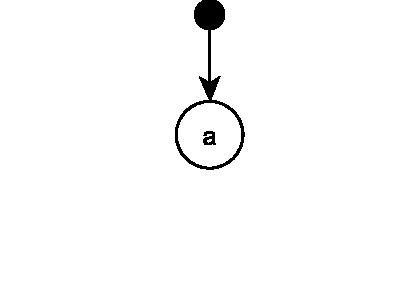
\includegraphics[width=\linewidth]{statechart_01}
        \caption{no-conflict}
        \label{fig:statechart_01}
    \end{subfigure}
    \hfill
    \begin{subfigure}[t]{0.49\linewidth}
        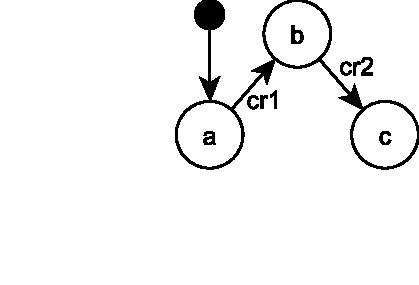
\includegraphics[width=\linewidth]{statechart_02}
        \caption{no-conflict}
        \label{fig:statechart_02}
    \end{subfigure}
    \begin{subfigure}[t]{0.49\linewidth}
        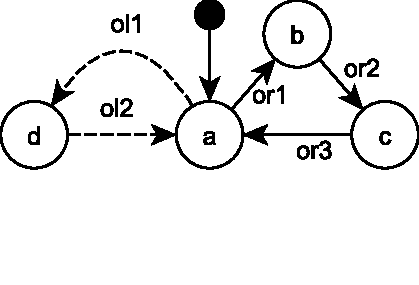
\includegraphics[width=\linewidth]{statechart_03}
        \caption{no-conflict}
        \label{fig:statechart_03}
    \end{subfigure}
    \hfill
    \begin{subfigure}[t]{0.49\linewidth}
        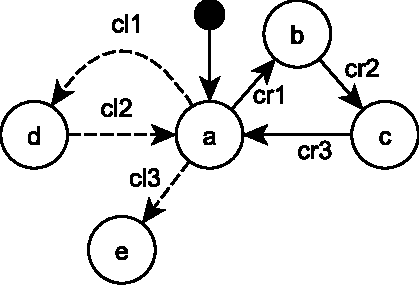
\includegraphics[width=\linewidth]{statechart_04}
        \caption{conflict}
        \label{fig:statechart_04}
    \end{subfigure}
    \begin{subfigure}[t]{0.49\linewidth}
        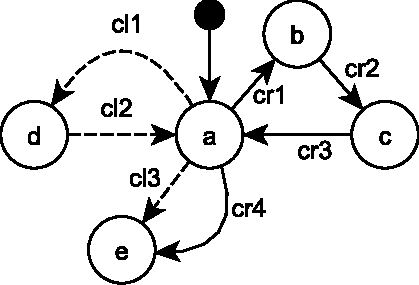
\includegraphics[width=\linewidth]{statechart_05}
        \caption{pseudo-conflict}
        \label{fig:statechart_05}
    \end{subfigure}
    \hfill
    \begin{subfigure}[t]{0.49\linewidth}
        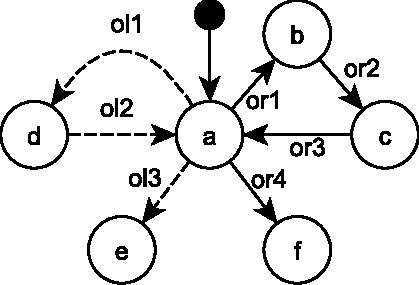
\includegraphics[width=\linewidth]{statechart_06}
        \caption{conflict}
        \label{fig:statechart_06}
    \end{subfigure}
    \caption{Conflicting and non-conflicting changes.}
    \label{fig:conflict_states}
\end{figure}




%Since only the last operation applied to an element that determines the element's eventual state, we can infer that the last operations $e_{ln}$ in $O_{L}$ and $e_{rm}$  in $O_{R}$, where $n$ = $|O_{L}|$ and $m$ = $|O_{R}|$, are the operations that are definitely in conflict. 
%\begin{equation} \label{eq:conflict_3.11}
%\begin{split}
%& e_{l} \not\equiv e_{r} \wedge n > 0 \wedge m > 0 \Rightarrow\\
%& o_{ln} \;!\; o_{rm}
%\end{split}
%\end{equation} 
%Nonetheless, since we also consider about resolving conflicts, a resolution of two conflicting operations that affect an element should also take into account all preceding operations applied to the element. This means picking one operation from one side as the applied operation does not only cancel the other side operation but also cancels all preceding operations that affected the element on the other side. Cancelling these operations set the element to its original state which makes all the chosen side operations can be applied safely -- avoiding further un-calculated conflicts with the rest of other side operations if we only cancel the last operation. 
%
%For example, let's say that  $o_{l1}$ =  [\texttt{\small \textbf{set} x.name \textbf{from} "A" \textbf{to} "B"}] on the left side, and it is also set twice consecutively -- $o_{r1}$ = [\texttt{\small \textbf{set} x.name \textbf{from} "A" \textbf{to} "C"}] and$o_{r2}$ = [\texttt{\small \textbf{set} x.name \textbf{from} "C" \textbf{to} "D"}] -- on the right side. Both operations $o_{r1}$ and $o_{r2}$ are in conflict if we use (\ref{eq:conflict_3.11}). Cancelling operation $o_{r2}$ does not have any affect in resolving the conflict since operation $o_{r1}$ are still in conflict with operation $o_{l1}$. 



\IncMargin{1.5em}
\begin{algorithm*}
    \begin{scriptsize}
        \SetKwInOut{Input}{input}
        \SetKwInOut{Output}{output}
        \Input{an instance of ElementTree $elementTree$}
        \Begin{
            $conflictList$ $\leftarrow$ ConflictList()\;
            \ForEach{$element$ \In $elementTree$}{
                \tcp{Handle conflicts with deletion ----------------------------}
                \If{isLeftDeleted($element$) \Or isRightDeleted($element$)}{
                    $leftEvents$ $\leftarrow$ getAllRelatedLeftEvents($element$)\;
                    $rightEvents$ $\leftarrow$ getAllRelatedRightEvents($element$)\;
                    \If{size($leftEvents$) > 0 \AndA size($rightEvents$) > 0}{
                        $conflict$ $\leftarrow$ createConflict($leftEvents$, $rightEvents$)\;
                        \If{isLeftDeleted($element$) \AndA isRightDeleted($element$)}{
                            setPseudo($conflict$)\;
                        }
                        addConflict($conflict$, $conflictList$)\;
                    }
                }
                \tcp{Handle conflicts with cross-container move --------------------------}
                \If{(getOriginalContainer($element$) <> getLeftContainer($element$) \Or getOriginalContainingFeature($element$) <> getLeftContainingFeature($element$)) \Or
                    (getOriginalContainer($element$) <> getRightContainer($element$) \Or getOriginalContainingFeature($element$) <> getRightContainingFeature($element$))}{
                    $leftEvents$ $\leftarrow$ getAllRelatedLeftEvents($element$)\;
                    $rightEvents$ $\leftarrow$ getAllRelatedRightEvents($element$)\;
                    \If{size($leftEvents$) > 0 \AndA size($rightEvents$) > 0}{
                        $conflict$ $\leftarrow$ createConflict($leftEvents$, $rightEvents$)\;
                        \If{getLeftContainer($element$) = getRightContainer($element$) \AndA getLeftContainingFeature($element$) = getRightContainingFeature($element$}{
                            setPseudo($conflict$)\;
                        }
                        addConflict($conflict$, $conflictList$)\;
                    }
                }
                \ForEach{$feature$ \In getFeatures($element$)}{
                    \tcp{Handle single-valued feature --------------------------}
                    \uIf{isSingleValued($feature$)}{
                        $originalValue$ $\leftarrow$ getOriginalValue($feature$)\;
                        $leftValue$ $\leftarrow$ getLeftValue($feature$)\;
                        $rightValue$ $\leftarrow$ getRightValue($feature$)\;
                        $leftEvents$ $\leftarrow$ getAllRelatedLeftEvents($element$, $feature$)\;
                        $rightEvents$ $\leftarrow$ getAllRelatedRightEvents($element$, $feature$)\;
                        \If{$originalValue$ <> $leftValue$ \Or $originalValue$ <> $rightValue$ \AndA size($leftEvents$) > 0 \AndA size($rightEvents$) > 0}{
                            $conflict$ $\leftarrow$ createConflict($leftEvents$, $rightEvents$)\;
                            \If{ $leftValue$ = $rightValue$}{
                                setPseudo($conflict$)\;
                            }
                            addConflict($conflict$, $conflictList$)\;
                        }
                    }
                    \tcp{Handle multi-valued feature --------------------------}
                    \ElseIf{isMultiValued($feature$)}{
                        \uIf{isOrdered($feature$)}{
                            $values$ $\leftarrow$ getUnequalLeftAndRightValues($feature$)\;
                            \ForEach{$value$ \In $values$}{
                                $leftEvents$ $\leftarrow$ getAllRelatedLeftEvents($element$, $feature$, $value$)\;
                                $rightEvents$ $\leftarrow$ getAllRelatedRightEvents($element$, $feature$, $value$)\;
                                \If{size($leftEvents$) > 0 \AndA size($rightEvents$) > 0}{
                                    $conflict$ $\leftarrow$ createConflict($leftEvents$, $rightEvents$)\;
                                    \If{getLeftIndex($value$, $feature$) = getRightIndex($rightValue$, $feature$)}{
                                        setPseudo($conflict$)\;
                                    }
                                    addConflict($conflict$, $conflictList$)\;
                                }       
                            }
                        }\ElseIf{\Not isOrdered($feature$)}{
                            $values$ $\leftarrow$ getXORLeftAndRightValues($feature$)\;
                            \ForEach{$value$ \In $values$}{
                                $leftEvents$ $\leftarrow$ getAllRelatedLeftEvents($element$, $feature$, $value$)\;
                                $rightEvents$ $\leftarrow$ getAllRelatedRightEvents($element$, $feature$, $value$)\;
                                \If{size($leftEvents$) > 0 \AndA size($rightEvents$) > 0}{
                                    $conflict$ $\leftarrow$ createConflict($leftEvents$, $rightEvents$)\;
                                    \If{isExisted($value$, $feature$) = isExisted($rightValue$, $feature$)}{
                                        setPseudo($conflict$)\;
                                    }
                                    addConflict($conflict$, $conflictList$)\;
                                }       
                            }
                        }
                    }
                }
            }
            \Return{$conflictList$}\;
        }
    \end{scriptsize}
    \caption{Algorithm for conflict detection using element tree.}
    \label{alg:conflict_detection}
\end{algorithm*}
\DecMargin{1.5em}


\subsection{Procedure for Detecting Conflicts} 
\label{sec:procedure_for_detecting_conflicts} 
We perform procedure in Alg. \ref{alg:conflict_detection} and employ (\ref{eq:conflict_3.3}) and (\ref{eq:conflict_3.4}) inside it to identify conflicts between two CBPs. Basically, the algorithm works by iterating through all the elements, features, and values in the element three (Fig. \ref{fig:element_tree_game}) and checking the equivalency of their original and eventual states as well the numbers of operations applied to them. The results are then used as inputs to decide whether a conflict has been detected or not.

The algorithm starts by creating a empty list \textsf{conflictList} to contain identified conflicts (lines 2). 
The algorithm then iterates through all the elements, features, and values in the element three. 
At lines 4 to 11, the algorithm checks if there is a conflict related to a deletion of an element.
If an element is deleted on one side or both sides, it means that all events related to the element on both sides should be in conflict. 
To get all the related events, the algorithm use functions \textsf{getAllRelatedLeftEvents(element)} 
and \textsf{getAllRelatedLeftEvents(element)} (elementact as a map key to access the events) that return two sets of the related events, 
\textsf{leftEvents} and \textsf{rightEvents} respectively. The related events are events applied to the deleted element, including its sub-elements and features, 
and events that are parts of composite events. If both sets of events are not empty then a conflict is created containing both sets of events. 
If the element is deleted on both sides then we set the conflict as \textsf{PSEUDO}. The identified conflict is then added to \textsf{conflictList}.

\begin{table*}[ht]
    \centering
    \caption{Conflicting change events in Listings \ref{lst:cbp_right} and \ref{lst:cbp_left} identified using the proposed conflict detection.}
    \label{table:conflicts_cbp}
    \begin{tabular}{|l|l|l|l|}
        \hline
        \multicolumn{1}{|c|}{{\color[HTML]{000000} \textbf{ID}}} & \multicolumn{1}{c|}{{\color[HTML]{000000} \textbf{Left Change Events (Bob)}}}                                                                                                                            & \multicolumn{1}{c|}{{\color[HTML]{000000} \textbf{Right Change Events (Alice)}}}                                                                                                                  & \multicolumn{1}{c|}{{\color[HTML]{000000} \textbf{Type}}}                 \\ \hline
        CB1                                                      & set troll.name from "Troll" to "Ogre"                                                                                                                                                                    & set troll.name from "Troll" to "Orc"                                                                                                                                                              & \begin{tabular}[c]{@{}l@{}}non-\\ commutability\end{tabular}              \\ \hline
        CB2                                                      & move target in character.parameters from 1 to 2                                                                                                                                                          & move target in character.parameters from 1 to 0                                                                                                                                                   & \begin{tabular}[c]{@{}l@{}}non-\\ commutability\end{tabular}              \\ \hline
        CB3                                                      & \begin{tabular}[c]{@{}l@{}}unset cast.name from "cast" to null\\ remove cast from giant.operations at 0\\ delete cast type Operation\\ unset giant.name from "Giant" to null\\ delete giant\end{tabular} & \begin{tabular}[c]{@{}l@{}}remove cast from giant.operations at 0\\ add cast to mage.operations at 0\\ remove smash from knight.operations at 0\\ add smash to giant.operations at 1\end{tabular} & \begin{tabular}[c]{@{}l@{}}non-\\ applicability,\\ composite\end{tabular} \\ \hline
        CB4                                                      & set character.name from "Character" to "Hero"                                                                                                                                                                    & set character.name from "Character" to "Hero"                                                                                                                                                              & \begin{tabular}[c]{@{}l@{}}pseudo, non-\\ commutability\end{tabular}              \\ \hline
    \end{tabular}
\end{table*}


\subsubsection{Conflict with Deletion} 
\label{sec:delete_conflict} 
As an example, when the iteration reach element \textsf{giant}, the algorithm identifies that the element has been deleted only on the left side.
The algorithm then collects all the related events from both. 
The left events consist of all events as parts of the deletion of element \textsf{giant} composite event. 
The right events consist of events that remove operation \textsf{smash} from class \textsf{knight} and add it to class \textsf{giant} and events 
that remove operation \textsf{cast} from class \textsf{giant} to class \textsf{mage}. The algorithm then creates an conflict that consists of these events 
producing conflict \textsf{CB3} in Table \ref{table:conflicts_cbp}. The conflict is not set \textsf{PSEUDO} since the element is only deleted on the left side. 

\subsubsection{Conflict between Cross-container Moves} 
\label{sec:move_conflict} 
Lines 15 to 25 are dedicated to identify conflicts related to cross-container moves. 
First, the algorithm checks if an element has been moved from its original container to another container, on one of the sides or both sides. 
If only on one side or both sides the element has been moved to another container, 
it continues to check the number of events related to the element by firstly obtaining change events related to the element on 
both sides using functions \textsf{getAllRelatedLeftEvents($element$)} and \textsf{getAllRelatedLeftEvents($element$)} yielding two sets of events, 
\textsf{leftEvents} and \textsf{rightEvents}. If the element has, at least, one event on each side,
a conflict is created containing \textsf{leftEvents} and \textsf{rightEvents}. 
If on both sides the element is moved to the same container then the conflict is set to \textsf{PSEUDO}. The conflict is then added to \textsf{conflictList}. 

\subsubsection{Single-valued Feature Conflict} 
\label{sec:single_valued_conflict}
Similar procedure also applies to single-valued features (lines 27-39). The procedure starts by retrieving \textsf{leftValue}, \textsf{rightValue}, and \textsf{originalValue} of a single-valued feature. It then checks the inequality of \textsf{leftValue} and \textsf{rightValue} to \textsf{originalValue}. If one of \textsf{leftValue} and \textsf{rightValue} are not equal to \textsf{originalValue}, it then continues to check the number of change events related to the feature by firstly retrieving them using function \textsf{getAllRelated*Events($element$, $feature$)} (element and feature act as a map key to access the events) yielding two sets of related events, \textsf{leftEvents} and \textsf{rightEvents}. If \textsf{leftEvents} and \textsf{rightEvents} are not empty then a conflict that contains these events is instantiated. The procedure then checks the equality of \textsf{leftValue} and \textsf{rightValue} and set the conflict to \textsf{PSEUDO} if \textsf{leftValue} and \textsf{rightValue} are equal. Finally, the conflict is put into \textsf{conflictList}. 

For example, when the iteration reach feature \textsf{name} of class \textsf{troll}, the algorithm retrieves the left, right, and original values of the feature, yielding ``Ogre'', ``Orc'', and ``Troll'' respectively. Since ``Ogre'' and Orc'' are not equal to ``Troll'', the algorithm continues to retrieve two sets of events related to the feature. Only one event contained exists in each set. On the left side, the event sets the name of class \textsf{troll} from ``Troll'' to ``Ogre'', while on the right side, the the event sets it from ``Troll'' to ``Orc''. Both event sets are not empty thus a conflict containing them is created. Since ``Ogre'' is not equal to ``Orc'' the conflict is not set to \textsf{PSEUDO}. This conflict is the conflict \textsf{CB1} in Table \ref{table:conflicts_cbp}. This part of the algorithm also identifies conflict \textsf{CB4} except that this conflict is set to \textsf{PSEUDO} since both sides change class \textsf{character}'s \text{name} to ``Hero''.   

\subsubsection{Ordered Multi-valued Feature Conflict} 
\label{sec:ordered_conflict}
Conflict detection for ordered, multi-valued features (lines 41 to 53) relies on function \textsf{getUnequalLeftAndRightValues}. The function returns all values from left and right sides that are not equal to their original states in terms of (in)existence and indexes. For example, in Fig. \ref{fig:element_tree_game}, parameter \textsf{target} in feature \textsf{parameters} is at index 2 on the left side but at index 1 in its original state. Thus, the value is included in the returned set. On the right side, this parameter is also at different index to its original index but it is already included the returned set. 

The algorithm then iterates through the values of the set. For each value, it retrieves all events related to the value on this feature (element, feature, and value act as a map key to access the events) using function \textsf{getAllRelated*Events($element$, $feature$, $value$)} yielding two sets of events, \textsf{leftEvents} and \textsf{rightEvents}. If both sets of events are not empty then a conflict is created. If the value on both sides is at the same index then the conflict is \textsf{PSEUDO}. Lastly, the conflict is added to \textsf{conflictList}. The parameter \textsf{target} in feature \textsf{parameters} has been concurrently modified; it has one event on each side: parameter \textsf{target} is moved to the last index on the left side and to the first index on the right. Thus, a conflict in detected. This conflict is presented as conflict \textsf{CB2} in Table \ref{table:conflicts_cbp}.


\begin{figure}
    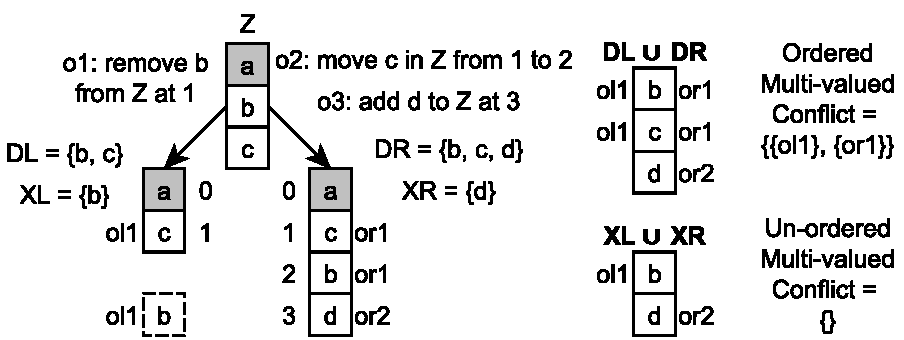
\includegraphics[width=\linewidth]{multi_valued_conflict_detection}
    \caption{Detecting conflicts in Multi-valued features ($D$: values that are different at every index; $X$: XOR of values).}
    \label{fig:multi_valued_conflict_detection}
\end{figure}

\subsubsection{Unordered Multi-valued Feature Conflict} 
\label{sec:unordered_conflict}
Conflict detection for un-odered, multi-valued features is handled at lines 54 to 67. Instead of using function \textsf{getUnequalLeftAndRightValues}, it employs function \textsf{getXORLeftAndRightValues}. The function also returns all values from left and right sides that are not equal to their original states but only in terms of (in)existence since indexing is not considered in un-ordered features. The procedure to detect a conflict is similar to the procedure for ordered features except that it check the existence of values (function \textsf{isExisted}) to determine if a conflict is \textsf{PSEUDO} or not.

\begin{figure*}
    \begin{tabular}{l|c|r}
        \begin{subfigure}[t]{0.31\linewidth}
            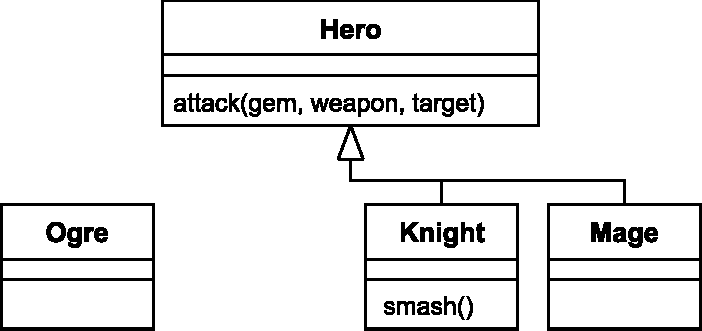
\includegraphics[width=\linewidth]{class_diagram_merged_ecbp}
            \caption{Epsilon CBP}
            \label{fig:class_diagram_merged_ecbp}
        \end{subfigure}
        &
        \begin{subfigure}[t]{0.31\linewidth}
            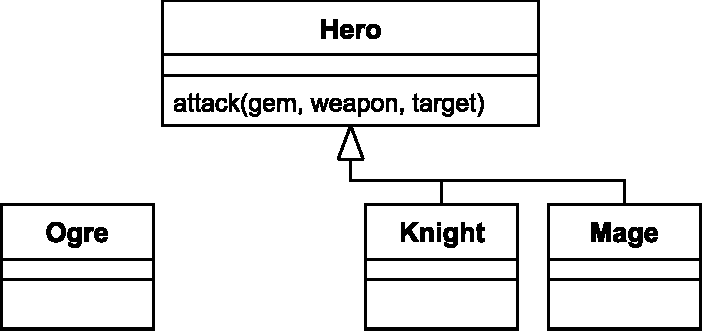
\includegraphics[width=\linewidth]{class_diagram_merged_emfc}
            \caption{EMF Compare}
            \label{fig:class_diagram_merged_emfc}
        \end{subfigure}
        &
        \begin{subfigure}[t]{0.31\linewidth}
            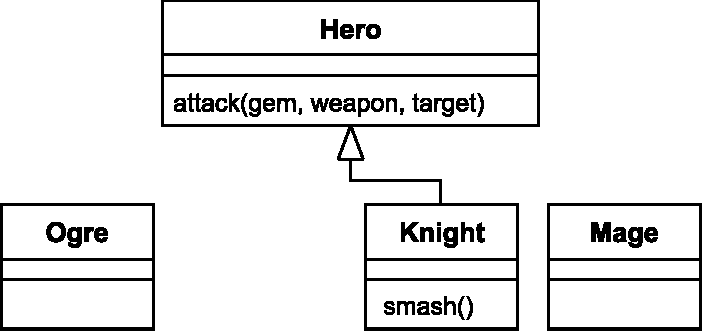
\includegraphics[width=\linewidth]{class_diagram_merged_emfs}
            \caption{EMF Store}
            \label{fig:class_diagram_merged_emfs}
        \end{subfigure}
    \end{tabular}
    \caption{Merged models of models in Fig. \ref{fig:class_diagram_rpg} after applying all-left-to-right merging.}
    \label{fig:class_diagram_merged}
\end{figure*}

\section{Merging}
\label{sec:merging}
Conflict resolution and merging strategies are out of the scope of this paper. However, it is important to present the merged models of these three approaches in order inspect their correctness. Thus, we present the merged models of the models in Fig. \ref{fig:class_diagram_rpg} using these three different approaches. The merge is all-left-to-right merge which means the left changes is prioritised above right changes. In other words, the right changes is applied first to the original model so that the left changes can override the right changes. If there is a conflict then the conflicting right changes are cancelled. In EMF Compare, this cancellation means only the left changes are executed, the right changes are \emph{not executed}, while, in Epsilon CBP and EMF Store, the right changes are \emph{reversed} so that the affected elements are brought back to their original states.    

In the default implementation of EMF Compare, the all-left-to-right merge sets the right model as the target and the left model as the source. This means the left changes are not applied to the original model. Instead, they are applied to the right model. Using this strategy, if we resolve all the conflicts in Table \ref{table:conflicts_emfc} using the all-left-to-right merge, we get a merged model as in Fig. \ref{fig:class_diagram_merged_emfc}. All the right events are not executed. Instead, in the right model, class \textsf{character}'s feature \text{name} is set to ``Hero'' and class \textsf{troll}'s feature \textsf{name} is set to ``Ogre''. Also, operation \textsf{cast} and class \textsf{giant} are removed from the right model. The removal of class \textsf{giant} also removes operation \textsf{smash} since the operation is contained by the class in the right model. 

For Epsilon CBP and EMF Store, applying the all-left-to-right merging requires all the right events of the conflicts in Tables \ref{table:conflicts_emfs} and \ref{table:conflicts_cbp} to be reversed. This reversal brings back the states of the elements affected by the conflicting right events to their original states which makes the conflicting left events safe to be applied to the original model. All right events are applied first followed by the reversed conflicting right events and then by all left events (see Listings \ref{lst:cbp_merged_emfs} and \ref{lst:cbp_merged_ecbp}). In this order, the events are applied to the original model, not the right model as in the EMF Compare, to produce the merged model.

\begin{lstlisting}[firstnumber=1,style=eol,caption={Merged change events (operations) of the models in Fig. \ref{fig:class_diagram_rpg} and Listings \ref{lst:cbp_right} and \ref{lst:cbp_left} using EMF Store. The commented lines are added only to improve readability.},label=lst:cbp_merged_emfs]
#--right events--
move target in attack.parameters from 1 to 0
remove smash from knight.operations at 0 composite l1
add smash to giant.operations at 0 composite l1
remove cast from giant.operations at 1 composite l2
add cast to mage.operations at 0 composite l2
create rightGen type Generalization
set rightGen.general to character
set troll.generalization to rightGen
set character.name from "Character" to "Hero"
remove rightGen from troll.generalization composite l3
set mage.generalization to rightGen composite l3
set troll.name from "Troll" to "Orc"
#--reversed conflicting right events--
set troll.name from "Orc" to "Troll"
remove rightGen from mage.generalization composite l3r
set troll.generalization to rightGen composite l3r
set character.name from "Hero" to "Character"
remove rightGen from troll.generalization
set rightGen.general from character to null
delete rightGen
remove cast from mage.operations at 0 composite l2r
add cast to giant.operations at 1 composite l2r
remove smash from giant.operations at 0 composite l1r
add smash to knight.operations at 0 composite l1r
move target in attack.parameters from 0 to 1
#--left events--
create leftGen type Generalization
set leftGen.general to character
set troll.generalization to leftGen
set character.name from "Character" to "Hero"
remove leftGen from troll.generalization composite r1
set knight.generalization to leftGen composite r1
move target in attack.parameters from 1 to 2
unset cast.name from "cast" to null composite r2
remove cast from giant.operations at 0 composite r2
delete cast composite r2
unset giant.name from "Giant" to null composite r2
delete giant comp r2
set troll.name from "Troll" to "Ogre"
\end{lstlisting}

\vspace{-20pt}
\begin{lstlisting}[firstnumber=1,style=eol,caption={Merged change events (operations) of the models in Fig. \ref{fig:class_diagram_rpg} and Listings \ref{lst:cbp_right} and \ref{lst:cbp_left} using Epsilon CBP. The commented lines are added only to improve readability.},label=lst:cbp_merged_ecbp]
#--right events--
move target in attack.parameters from 1 to 0
remove smash from knight.operations at 0 composite l1
add smash to giant.operations at 0 composite l1
remove cast from giant.operations at 1 composite l2
add cast to mage.operations at 0 composite l2
create rightGen type Generalization
set rightGen.general to character
set troll.generalization to rightGen
set character.name from "Character" to "Hero"
remove rightGen from troll.generalization composite l3
set mage.generalization to rightGen composite l3
set troll.name from "Troll" to "Orc"
#--reversed conflicting right events--
set troll.name from "Orc" to "Troll"
remove cast from mage.operations at 0 composite l2r
add cast to giant.operations at 1 composite l2r
remove smash from giant.operations at 0 composite l1r
add smash to knight.operations at 0 composite l1r
move target in attack.parameters from 0 to 1
#--left events--
create leftGen type Generalization
set leftGen.general to character
set troll.generalization to leftGen
set character.name from "Character" to "Hero"
remove leftGen from troll.generalization composite r1
set knight.generalization to leftGen composite r1
move target in attack.parameters from 1 to 2
unset cast.name from "cast" to null composite r2
remove cast from giant.operations at 0 composite r2
delete cast composite r2
unset giant.name from "Giant" to null composite r2
delete giant comp r2
set troll.name from "Troll" to "Ogre"
\end{lstlisting}

The drawback of the EMF Compare approach is that it set the right model as the target for merging changes resulting the lost of operation \textsf{smash} in the merged model (Fig. \ref{fig:class_diagram_merged_emfc}). In contrast, Epsilon CBP and EMF Store reverse the event that moves operation \textsf{smash} from class \textsf{knight} to class \textsf{giant} so that it moves back operation \textsf{smash} from class \textsf{giant} to class \textsf{knight}. The drawback of EMF Store is that it does not concern about the eventual states produced by the conflicting events. It only concern that a feature has been modified concurrently on both sides identified by the presence of, at least, an event on each side. For example, the eventual states of class \textsf{troll}'s feature \textsf{generalization} are \textsf{null} in the original, left, and right models. However, these are not considered by EMF Store. Instead, it only identifies that there are events on both sides associated to this feature. Thus, conflict \textsf{ES1} in \ref{table:conflicts_emfs} is generated. In consequence, all events related to the feature on the right side, and the events that are part of their composite events, are reversed resulting the exclusion of generalization \textsf{rightGen} from the merged model. This drawback has been addressed by the Epsilon CBP by checking the equality of the original, left, and right states of the feature. Since they are all equal then there is no conflict between the events. Thus, Epsilon CBP produces a merged model as in Fig. \ref{fig:class_diagram_merged_ecbp}.


\section{Evaluation Method}
\label{sec:evaluation}
In this section, we present the method that we employed to evaluate our change-based comparison approach and discuss the results. We also present the limitations and threats to the validity of the evaluation.

In order to assess the performance benefits of the change-based approach in terms of model comparison -- differencing and conflict detection, we have evaluated it against a mature and widely-used state-based comparison tool (EMF Compare \cite{emfcompare2018developer,eclipse2017compare}). Since there are no manually developed, large models persisted in our change-based format yet, the dataset for our experiments was constructed from a large model reverse-engineered from the Eclipse Epsilon project \cite{eclipse2018epsilongit,eclipse2017epsilon}. This model conforms to the Java metamodel \cite{eclipse2018modiscojava} and consists of more than 1.6 million elements with a size of 224 MBs when persisted in XMI. 

We cloned the original model to produce two new (left and right) models and perform operations (\textsf{add}, \textsf{remove}, \textsf{move}, \textsf{set} with random elements, features, indexes, and values) on both models to create differences. We made 1.1 million artificial changes to each model, generating over 1.1 million events (one operation can generate more than one event, e.g. a \textsf{move} between features generates \textsf{remove} and \textsf{add} events). Events generated by the changes were persisted in our change-based format (to be used later in change-based model comparison). After every 50,000 changes, we made a measurement point. We persisted the last state of the models in state-based format (to be used later in state-based model comparison) and then performed change-based and state-based model comparison and measured their execution time and memory footprint. We created 22 measurement points to capture their trends in one experiment. 

\subsection{Model Differencing}
\label{sec:differencing_evaluation}

We conducted five experiments to evaluate the model differencing of our approach.
%batches \dk{Would it make sense to call these ``experiments'' instead? i.e. ``We conducted five experiments. In the first experiment \ldots''}. 
In the first experiment, the ratio of occurrence between \textsf{add}, \textsf{remove}, \textsf{move}, and \textsf{set} changes is set to 1:1:20:40 intuitively in assumption that in a mature model modification -- \textsf{move} and \textsf{set} events -- occurs more frequent than addition and deletion. Since we wanted the change of total elements not to affect our measurement, the number of total elements should be kept constant. For example, it is difficult to tell an increase of time in comparison is caused by an increase in the number of elements or by the number of change events. One way to do this was to exclude \textsf{add} and \textsf{remove} operations. However, excluding both operations made measurement less representative. Thus, we still included both operations but made their probabilities equal so that the number of total elements remain largely unchanged. In the rest of the experiments,
%batches \dk{Replace with ``In the remaining four experiments''? - it may not be entirely clear to the reviewers what ``to support'' means in this context}
we only performed homogeneous type operations -- isolated from other types -- per experiment (e.g. add-only, move-only operations). In the end, we obtained 5 results of the experiments: mixed, add-only, remove-only, move-only, and set-only measurement results. We did this to asses whether operations of different types have a different impact on model comparison.
%\dk{Explain that we did this to assess whether events of different types have a different impact on model comparison?}

For the change-based approach, the comparison time comprises loading change events, constructing an element tree, and identifying differences. The memory footprint is the space used to hold the change events, element tree, and differences in memory. For the state-based approach, the comparison time comprises matching elements and identifying differences, and the memory footprint is the space required to hold the matches and differences in memory. All measurements were performed on the same machine with the following specification: AMD Opteron(tm) Processor 6386 SE @ 2.8 GHz cache size 2 GBs (64 processors), 528 GBs main memory, Ubuntu 16.04.6 LTS operating system, and Java(TM) SE Runtime Environment (build 1.8.0\_201-b09) with JVM \textsf{InitialHeapSize} 2GBs and \textsf{MaxHeapSize} 32 GBs.
%\dk{Add the spec of the machine + the version of Java used + how much memory was allocated to the JVM}

Since the change-based and state-based approaches can produce a different number of syntactically equivalent differences, in order to evaluate the correctness of the change-based approach, we reconciled all the differences by performing all-left-to-right merging -- making the right model identical to the left model -- based on the identified differences. If the all-left-to-right merging of change-based approach produces a model that is identical to the model produced by the all-left-to-right merging of the state-based approach then it can be said that differences identified by the change-based approach are correct. We performed this correctness checking at every measurement point.

\subsection{Conflict Detection}
\label{sec:conflict_detection_evaluation}
In evaluating our conflict detection approach, basically we followed the similar procedures as in the model differencing evaluation, except that we add another implementation of change-based model persistence (EMF Store \cite{koegel2010emfstore}) to compare it with our approach. We did not include it in the model differencing evaluation since it works purely on operations, and it is designed to identify conflict between operations; not for finding differences between models. We imported the changes persisted in our change-based format into EMF Store by replaying the changes in the EMF Store. Thus, we could obtain equivalent changes but in the EMF Store format. Since in this evaluation we used two change-based persistence: our approach and EMF Store, we use the term Epsilon CBP to refer to our approach. Due to slow execution of replaying \textsf{delete} event in EMF Store, we have to reduce the size of the models to 70 thousand elements each and the number of changes to 550 thousands with 25 thousand changes for each measurement point -- 22 measurement points in total.

\begin{figure*}[ht]
    %    \vspace{-26pt}
    \begin{subfigure}[]{0.33\linewidth}
        \includegraphics[width=\linewidth]{mixed-count-events}
        \caption{total elements, affected elements, and diffs}
        \label{fig:modification_course}
    \end{subfigure}
    \begin{subfigure}[]{0.33\linewidth}
        \includegraphics[width=\linewidth]{mixed-time-events}
        \caption{execution time}
        \label{fig:time_diffs}
    \end{subfigure}
    \begin{subfigure}[]{0.33\linewidth}
        \includegraphics[width=\linewidth]{mixed-memory-events}
        \caption{memory footprint}
        \label{fig:memory_diffs}
    \end{subfigure}
    \caption{Change-based vs. state-based model comparison as change events increase.}
    \label{fig:change_vs_state}
\end{figure*}

\vspace{-5pt}
\section{Evaluation Results and Discussion}
\label{sec:discussion}
In this section, we report on the obtained results in terms of comparison time and memory footprint for both model differencing and conflict detection. 


\subsection{Model Differencing}
\label{sec:differencing_results}
This section presents the results of both mixed and homogeneous operation measurements for the model differencing evaluation. 

\vspace{-5pt}
\subsubsection{Mixed Operations} \label{sec:mixed-operation}

In the mixed operation measurement, we modify two identical models differently by applying random operations. As the number of change events generated by the modification grows, the numbers of affected elements and differences also increase in a logarithmic manner. The patterns can be seen in Fig. \ref{fig:modification_course}. The growth is logarithmic since the probability that the random operations modify the same elements also increases. Thus, some change events might not contribute to the addition of new affected elements and differences. In other words, more events are required to increase the number of affected elements or differences. In Fig. \ref{fig:modification_course}, the total elements remains largely unchanged due to the equal probabilities of addition and deletion as has been set in Section \ref{sec:evaluation}. The figure gives us an insight about the characteristics of the modification caused by the random operations in the mixed operation measurement; it supports explaining the implication of the changes on execution time and memory footprints of model comparison.

After applying some random changes on both models, the modification produces 100,000 change events at the first measurement point. Using this amount of events, our change-based comparison only takes 5 seconds to identify around 90,000 differences, in contrast to the state-based comparison that takes 66 seconds (see the first measurement points in Figures \ref{fig:modification_course} and \ref{fig:time_diffs}). If the modification continues, more changes events are generated. This growing number of change events has to be loaded into memory and thus slows down the change-based comparison. Nevertheless, the change-based comparison is still faster than the state-based comparison even though the number of change events reaches 2.37 millions -- more than 1 million differences at that point; the change-based comparison outperforms the state-based comparison in execution time (Figure \ref{fig:time_diffs}). Fig. \ref{fig:time_changediff_detail} breaks down the comparison time in detail. It exhibits that the event loading time is the dominant contributor to the slowdown compared to the element tree's construction time and diffing time. 

\begin{figure*}[ht]
    \centering
    \begin{subfigure}[t]{0.245\linewidth}
        \includegraphics[width=\linewidth]{mixed-time-events-detail}
        \caption{change-based comparison time}
        \label{fig:time_changediff_detail}
    \end{subfigure}
    \hfill
    \begin{subfigure}[t]{0.245\linewidth}
        \includegraphics[width=\linewidth]{state-time-events-detail}
        \caption{state-based comparison time}
        \label{fig:time_statediff_detail}
    \end{subfigure}
    \hfill
    \begin{subfigure}[t]{0.245\linewidth}
        \includegraphics[width=\linewidth]{mixed-memory-events-detail}
        \caption{change-based memory footprint}
        \label{fig:memory_changediff_detail}
    \end{subfigure}
    \hfill
    \begin{subfigure}[t]{0.245\linewidth}
        \includegraphics[width=\linewidth]{state-memory-events-detail}
        \caption{state-based memory footprint}
        \label{fig:memory_statediff_detail}
    \end{subfigure}
    \caption{Breakdown view of comparison time and memory footprint in Figure \ref{fig:change_vs_state}.}
    \label{fig:time_memory_detail}
\end{figure*}

For the state-based comparison in Fig. \ref{fig:time_statediff_detail}, the comparison time only experiences a slight increase as the number of identified differences also grows.
%\dk{Change to ``grows''?}. 
This slight increase is contributed mainly by the diffing time, while the matching time tends to be constant due to the very small increase of the total elements (Figures \ref{fig:modification_course}).

Nevertheless, change-based comparison generally consumes more memory than the state-based comparison (see Figure \ref{fig:memory_diffs}). It only consumes less memory than its state-based counterpart when the number of events is less than 0.3 millions (around less than 0.25 million identified differences at that moment). Fig. \ref{fig:memory_changediff_detail} breaks down the memory footprint of change-based comparison into three factors: the loaded change events, element tree, and diffs. As modification continues, an increasing number of events is generated. These events have to be loaded into memory since they contain the required information for the construction of an element tree. The amount of space to keep these change events in memory grows linearly with their number. 

In contrast, the memory used for the element tree grows logarithmically. As the number of events increases, the probability that events modify already affected elements also increases. Thus, no additional memory allocation is required for the element tree. We can also notice that the element tree occupies most of the memory footprint since it mirrors the partial states -- elements, features, and values -- of the models that are affected by the changes. Moreover, in our technical implementation, a feature can have many instances -- one instance for each element (As a comparison, in the EMF implementation, there is only one instance for a feature. The feature is used as a key so that different elements can have the same feature that maps to different values simultaneously). This contributes to the large memory footprint used by the element three. The identified change-based diffs, the third factor, are the smallest factor that contributes to the memory footprint of the change-based comparison. 

For the state-based comparison in Fig. \ref{fig:memory_statediff_detail}, the memory footprint only grows slightly along the increase of differences. A large part of the memory footprint is used to represent the identified differences, while the memory used for matches tends to be constant as the changes of the total elements are very small -- less new elements means less memory needs to be allocated for new matches (Figures \ref{fig:modification_course}). 

\subsubsection{Homogeneous Operations}
\label{sec:homogeneous-operation}

\begin{figure*}[ht]
    \centering
    \begin{subfigure}[t]{0.245\linewidth}
        \includegraphics[width=\linewidth]{add-time-events}
        \caption{add-only}
        \label{fig:add-time-events}
    \end{subfigure}
    \hfill
    \begin{subfigure}[t]{0.245\linewidth}
        \includegraphics[width=\linewidth]{delete-time-events}
        \caption{delete-only}
        \label{fig:delete-time-events}
    \end{subfigure}
    \hfill
    \begin{subfigure}[t]{0.245\linewidth}
        \includegraphics[width=\linewidth]{move-time-events}
        \caption{move-only}
        \label{fig:move-time-events}
    \end{subfigure}
    \hfill
    \begin{subfigure}[t]{0.245\linewidth}
        \includegraphics[width=\linewidth]{change-time-events}
        \caption{change-only}
        \label{fig:change-time-events}
    \end{subfigure}
    \caption{Comparison time for homogeneous operations.}
    \label{fig:operation_time_events}
\end{figure*}

\begin{figure*}[ht]
    \centering
    \begin{subfigure}[t]{0.245\linewidth}
        \includegraphics[width=\linewidth]{add-memory-events}
        \caption{add-only}
        \label{fig:add-memory-events}
    \end{subfigure}
    \hfill
    \begin{subfigure}[t]{0.245\linewidth}
        \includegraphics[width=\linewidth]{delete-memory-events}
        \caption{delete-only}
        \label{fig:delete-memory-events}
    \end{subfigure}
    \hfill
    \begin{subfigure}[t]{0.245\linewidth}
        \includegraphics[width=\linewidth]{move-memory-events}
        \caption{move-only}
        \label{fig:move-memory-events}
    \end{subfigure}
    \hfill
    \begin{subfigure}[t]{0.245\linewidth}
        \includegraphics[width=\linewidth]{change-memory-events}
        \caption{change-only}
        \label{fig:change-memory-events}
    \end{subfigure}
    \caption{Memory footprint for homogeneous operations.}
    \label{fig:operation_memory_events}
\end{figure*}

Figures \ref{fig:operation_time_events} and \ref{fig:operation_memory_events} exhibit the comparison time and memory footprint of models that have been modified using homogeneous operations -- \textsf{add}, \textsf{remove}, \textsf{move}, or \textsf{set} only. We can notice that in all figures change-based comparison outperforms its state-based counterpart particularly when the number of change events is small relative to the size of the model. As the number of modifications grows, eventually change-based comparison becomes slower than state-based comparison. In our experiments, this happens when the number of events is greater than 4 million (Fig. \ref{fig:add-time-events}). Change-based comparison also becomes slower when the size of models shrinks (due to a large number of delete events) as depicted in Fig. \ref{fig:delete-memory-events} as the change-based comparison still needs to load these change events and construct its element tree; in contrast, deletion means less work for state-based comparison. In terms of memory footprint, change-based comparison only performs better than state-based comparison when the number of change events is less than 0.3 millions as depicted in Fig. \ref{fig:operation_memory_events}.

\subsection{Conflict Detection}
\label{sec:conflict_results}

\begin{figure*}[ht]
    \centering
    \begin{subfigure}[t]{0.245\linewidth}
        \includegraphics[width=\linewidth]{conflict-size-events}
        \caption{number of elements}
        \label{fig:conflict-size-events}
    \end{subfigure}
    \hfill
    \begin{subfigure}[t]{0.245\linewidth}
        \includegraphics[width=\linewidth]{conflict-count-events}
        \caption{number of conflicts}
        \label{fig:conflict-count-events}
    \end{subfigure}
    \hfill
    \begin{subfigure}[t]{0.245\linewidth}
        \includegraphics[width=\linewidth]{conflict-time-events}
        \caption{execution time}
        \label{fig:conflict-time-events}
    \end{subfigure}
    \hfill
    \begin{subfigure}[t]{0.245\linewidth}
        \includegraphics[width=\linewidth]{conflict-memory-events}
        \caption{memory footprint}
        \label{fig:conflict-memory-events}
    \end{subfigure}
    \caption{Epsilon CBP vs. EMF Compare vs. EMF Store comparison as change events increase.}
    \label{fig:conflict_events}
\end{figure*}

This section presents the results of the conflict detection evaluation. 

\subsubsection{Mixed Operations}
\label{sec:mixed-operation_conflict}
Similar to the results in the model differencing evaluation (Fig. \ref{fig:modification_course}), the growing number of change events in the conflict detection evaluation is also followed by the logarithmic increase of affected elements (Fig. \ref{fig:conflict-size-events}). The total number of both elements can also be kept relatively constant due to 1:1 ratio of \textsf{add} and \textsf{delete} operations' occurrence. These change events produce different numbers of conflicts for Epsilon CBP, EMF Compare, and EMF Store as can be seen in Fig. \ref{fig:conflict-count-events}. However, the numbers of conflicts detected are slightly different due to their distinct conflict detection approaches. 

Fig. \ref{fig:conflict-time-events} exhibits Epsilon CBP outperforms EMF Compare and EMF Store in terms of execution time in detecting conflicts. In a comparison of two models that involves 1.01 million elements in total and 1.3 millions change events (the last measurement point), Epsilon CBP takes only 6.7 seconds to detect all conflicts while EMF Compare requires 21.4 seconds to finish the conflict detection. Both conflict detections are faster than EMF Store that needs 1 minute and 34.6 seconds to complete detecting conflicts. Fig. \ref{fig:conflict-memory-events} also shows Epsilon CBP outmatches EMF Compare and EMF Store in terms of memory footprint in conflict detection. At the last measurement point, Epsilon CBP only consumes 5 GBs which is much lesser than EMF Compare and EMF Store that occupy around 16 and 26 GBs of memory footprint respectively.

Fig. \ref{fig:conflict_time_events} shows the detailed view of Epsilon CBP, EMF Compare, and EMF Store on the time required to complete conflict detection. As can be seen in the Fig. \ref{fig:ecbp-conflict-time-events}, Epsilon CBP takes most of the time used to load change events and construct element tree compared to the time it takes for identifying conflicts. In detecting conflicts, the Epsilon CBP does not requires to perform differencing since changes are already available in the form of change events Thus, the differencing is not included in the diagram. In EMF Compare, at the last measurement point, we can notice that the time taken for matching and identifying conflicts is less than 6 seconds each, which is smaller than the time used for identifying differences that is 12.6 seconds (Fig. \ref{fig:emfc-conflict-time-events}). The differencing takes a great portion of the time since it needs to derive differences twice; differences between left and original models and right and original models. The time for for matching and differencing tends to have only slight increase since the sizes of the models are set to be as constant as possible (Fig. \ref{fig:modification_course}). In contrast, the time for detecting conflicts tends to grow faster than both due to the increasing number of conflicting (derived) changes as the number of modification -- change events -- increases. In detecting conflicts, EMF Store allocates more than a half of the consumed time for identifying conflicts. The rest of the time is used for loading changes and mapping between affected elements and their ids (Fig. \ref{fig:emfs-conflict-time-events}). 

\begin{figure*}[ht]
    \centering
    \begin{subfigure}[t]{0.32\linewidth}
        \includegraphics[width=\linewidth]{ecbp-conflict-time-events}
        \caption{Epsilon CBP}
        \label{fig:ecbp-conflict-time-events}
    \end{subfigure}
    \hfill
    \begin{subfigure}[t]{0.32\linewidth}
        \includegraphics[width=\linewidth]{emfc-conflict-time-events}
        \caption{EMF Compare}
        \label{fig:emfc-conflict-time-events}
    \end{subfigure}
    \hfill
    \begin{subfigure}[t]{0.32\linewidth}
        \includegraphics[width=\linewidth]{emfs-conflict-time-events}
        \caption{EMF Store}
        \label{fig:emfs-conflict-time-events}
    \end{subfigure}
    \caption{Detailed view of Epsilon CBP vs. EMF Compare vs. EMF Store on the time required for conflict detection.}
    \label{fig:conflict_time_events}
\end{figure*}

In terms of memory footprint, Epsilon CBP allocates most of the memory space for element tree construction and the rest is for the loading change events and identifying conflicts (Fig. \ref{fig:ecbp-conflict-memory-events}). The reason for this is due to our technical implementation explained in Section \ref{sec:mixed-operation}. In EMF Compare (Fig. \ref{fig:emfc-conflict-memory-events})), the amount of memory used for matching and differencing only increases slightly due the sizes of the models that are set to be as constant as possible (Fig. \ref{fig:modification_course}). In contrast, the memory used for detecting conflict increases positively as the number of detected conflicts rises (Fig. \ref{fig:conflict-count-events}). For EMF Store, the amount of memory used for loading changes and mapping is slightly above the amount of memory for identifying differences (Fig. \ref{fig:emfs-conflict-memory-events}).

\begin{figure*}[ht]
    \centering
    \begin{subfigure}[t]{0.32\linewidth}
        \includegraphics[width=\linewidth]{ecbp-conflict-memory-events}
        \caption{Epsilon CBP}
        \label{fig:ecbp-conflict-memory-events}
    \end{subfigure}
    \hfill
    \begin{subfigure}[t]{0.32\linewidth}
        \includegraphics[width=\linewidth]{emfc-conflict-memory-events}
        \caption{EMF Compare}
        \label{fig:emfc-conflict-memory-events}
    \end{subfigure}
    \hfill
    \begin{subfigure}[t]{0.32\linewidth}
        \includegraphics[width=\linewidth]{emfs-conflict-memory-events}
        \caption{EMF Store}
        \label{fig:emfs-conflict-memory-events}
    \end{subfigure}
    \caption{Detailed view of Epsilon CBP vs. EMF Compare vs. EMF Store on the memory footprint for conflict detection.}
    \label{fig:conflict_memory_events}
\end{figure*}

\subsubsection{Homogenous Operations}
\label{sec:homogenous-operation_conflict}

\begin{figure*}[ht]
    \centering
    \begin{subfigure}[t]{0.245\linewidth}
        \includegraphics[width=\linewidth]{add-conflict-time-events}
        \caption{add-only}
        \label{fig:add-conflict-time-events}
    \end{subfigure}
    \hfill
    \begin{subfigure}[t]{0.245\linewidth}
        \includegraphics[width=\linewidth]{delete-conflict-time-events}
        \caption{delete-only}
        \label{fig:delete-conflict-time-events}
    \end{subfigure}
    \hfill
    \begin{subfigure}[t]{0.245\linewidth}
        \includegraphics[width=\linewidth]{move-conflict-time-events}
        \caption{move-only}
        \label{fig:move-conflict-time-events}
    \end{subfigure}
    \hfill
    \begin{subfigure}[t]{0.245\linewidth}
        \includegraphics[width=\linewidth]{change-conflict-time-events}
        \caption{change-only}
        \label{fig:change-conflict-time-events}
    \end{subfigure}
    \caption{Conflict detection time for homogeneous operations.}
    \label{fig:homgeneous_operation_time_events}
\end{figure*}

\begin{figure*}[ht]
    \centering
    \begin{subfigure}[t]{0.245\linewidth}
        \includegraphics[width=\linewidth]{add-conflict-memory-events}
        \caption{add-only}
        \label{fig:add-conflict-memory-events}
    \end{subfigure}
    \hfill
    \begin{subfigure}[t]{0.245\linewidth}
        \includegraphics[width=\linewidth]{delete-conflict-memory-events}
        \caption{delete-only}
        \label{fig:delete-conflict-memory-events}
    \end{subfigure}
    \hfill
    \begin{subfigure}[t]{0.245\linewidth}
        \includegraphics[width=\linewidth]{move-conflict-memory-events}
        \caption{move-only}
        \label{fig:move-conflict-memory-events}
    \end{subfigure}
    \hfill
    \begin{subfigure}[t]{0.245\linewidth}
        \includegraphics[width=\linewidth]{change-conflict-memory-events}
        \caption{change-only}
        \label{fig:change-conflict-memory-events}
    \end{subfigure}
    \caption{Conflict detection memory for homogeneous operations.}
    \label{fig:homgeneous_operation_memory_events}
\end{figure*}

\begin{figure*}[ht]
    \centering
    \begin{subfigure}[t]{0.245\linewidth}
        \includegraphics[width=\linewidth]{add-conflict-count-events}
        \caption{add-only}
        \label{fig:add-conflict-count-events}
    \end{subfigure}
    \hfill
    \begin{subfigure}[t]{0.245\linewidth}
        \includegraphics[width=\linewidth]{delete-conflict-count-events}
        \caption{delete-only}
        \label{fig:delete-conflict-count-events}
    \end{subfigure}
    \hfill
    \begin{subfigure}[t]{0.245\linewidth}
        \includegraphics[width=\linewidth]{move-conflict-count-events}
        \caption{move-only}
        \label{fig:move-conflict-count-events}
    \end{subfigure}
    \hfill
    \begin{subfigure}[t]{0.245\linewidth}
        \includegraphics[width=\linewidth]{change-conflict-count-events}
        \caption{change-only}
        \label{fig:change-conflict-count-events}
    \end{subfigure}
    \caption{Conflict detection count for homogeneous operations.}
    \label{fig:homgeneous_operation_count_events}
\end{figure*}

Based on the findings in model differencing and conflict detection evaluation, we argue that the change-based comparison approach works at its best for large models that have been modified a moderate number of times. Models that have been excessively modified and experience significant reduction on model size could impair the performance of change-based comparison as a great number of change records have to be read and loaded into memory. 

\subsection{Limitations and Validity}
\label{sec:limitation_and_Threat_to_validity_7}
The evaluation of the proposed change-based comparison is limited to the Java metamodel only. Thus, there is no guarantee it will perform in a consistent manner on models conforming to different metamodels. Although, we have tried to cover as much as common changes made in EMF models (e.g. performing \textsf{add}/\textsf{remove}/\textsf{set}/\textsf{move} operations on \textsf{single}/\textsf{multi}-\textsf{valued} features, \textsf{attribute}/\textsf{reference} features, or \textsf{containment}/\textsf{non}-\textsf{containment} references), the random modification made in the evaluation does not largely reflect the evolution of models in the real world. This is challenging as different domains can have their own patterns of model evolution -- different problems, metamodels, modellers, etc.

\section{Related Work}
\label{sec:related_work}
We are not aware of any other work that targets comparison and diffing of change-based models persisted as files. There are however several existing tools for state-based model comparison. Beyond EMFCompare, which we used for our comparative evaluation due to its maturity and ongoing development activity, tools such as SiDiff \cite{Treude2007SiDiff} and DSMDiff \cite{lin2009dsmdiff} also provide language-agnostic graph-based model comparison, with some room for configuration (e.g. assigning different weights to features of types in the language). Additional expressive power -- at the cost of increased complexity and configuration effort -- is offered by dedicated comparison languages such as the Epsilon Comparison Language, which can be used to compare both homogeneous and heterogeneous models \cite{kolovos2009ecl}. We refrain from a more detailed discussion on state-based comparison tools as they all require upfront loading of both versions of the model into memory, which is the main cost that we aspire to reduce with the presented change-based approach.

Database-backed model persistence and version control solutions such as CDO \cite{eclipse2019cdo}, EMFStore \cite{koegel2010emfstore} also provide diffing capabilities between different versions of the same model without requiring models to be fully loaded into memory, however they present integration challenges with mainstream software engineering tools (e.g. continuous integration systems, backup and restore facilities) which are typically file-based, and their performance can degrade as more models/users are added to a repository, since all models are effectively stored in a single database \cite{KolovosRMPGCLRV13}.

\vspace{-10pt}
\section{Conclusions and Future Work}
\label{sec:conclusion_and_future_work}
In this paper, we have presented a novel approach to model comparison by exploiting the nature of change-based persistence which allows us to find differences between versions of a model by only comparing the last set of changes between the source and reference model.
Our evaluation results suggest that using this approach, we can produce model comparison that is faster than traditional, state-based model comparison.
However, the change-based comparison approach needs to load change events from a change-based persistence into main memory and thus may requires more memory than for state-based comparison. In our evaluation, this occurs when the number of change events exceeds 400,000.
Arguably, diff and merge operations are usually performed on smaller deltas than our evaluation.
The next challenge for future work is to identify strategies to merge models optimally and persist the merging in the change-based way. 
